\documentclass[11pt]{scrartcl}

\usepackage[utf8]{inputenc}
\usepackage[T1]{fontenc}
\usepackage{lmodern}

\usepackage[table]{xcolor} % tables
\usepackage{booktabs} % topline, midline, bottomline
\usepackage{graphicx} % PNG
\usepackage{float} % PNG location force
\usepackage{url}
\usepackage{pgf-umlcd} % Class diagrams
\usepackage{pgfplots} % diagrams
\usepackage{comment}
\usepackage{caption} 
\usepackage{subcaption} % mutiple captions beside each other
\usepackage{wrapfig} % text beside figures
\usepackage{tabu} % rowfont command in tables


\pgfplotsset{compat=newest}

\usepackage[english]{babel}
\usepackage{csquotes}
\usepackage{hyperref} % URLs

\setlength\doublerulesep{5pt} 


\title{Racism in the housing market}
\subtitle{Technical Writeup}
\author{
    Michael Brauweiler\\
    \and
    Vadim Goryainov\\
}
\date{\footnotesize Technical University of Munich\\\smallskip\today
%\\[\baselineskip] \today
}

\begin{document}
\maketitle
\begin{abstract} \small
    The goal of our project is to research the latent racism a person might encounter while searching for accommodation. We wanted to analyse whether persons with a foreign name are less likely to get a positive response to an application for accommodation than the ones with a German name and whether this response rate is correlated with the local support of populist parties. To acquire the data, we wrote a tool that sent automated requests to hundreds of offers on the website \url{www.wg-gesucht.de} in seven German cities. Thus we could show, that there is indeed a correlation between your name and your success in finding accommodation. Also, a correlation with local support for the political party \textit{AfD} is shown.
\end{abstract}

\section{The Automated Tool}
\begin{figure}[H]
\centering
    \includegraphics[width=.73\textwidth]{images/DataFlow.png}
    \caption{UML Data Flow Diagram}
    \label{fig:data_flow}
\end{figure}

\subsection{Setup and Workflow}
\label{sec:setup}

Our tool consists of several components that are executed in sequential order (see \textit{Figure} \ref{fig:data_flow}). The results of each component are saved on the hard drive and not only on the main memory. This allowed us to shutdown the program after running several components, check the interim results and resume the procedure. It also made sure that the results were not lost in case of an unexpected crash of the program - this was especially important as the tool runs for several hours per city. \newline
One big issue while crawling \url{www.wg-gesucht.de} and sending automated requests to the offers found was to avoid detection as a web bot by the website. For that reason we made a component \textsc{StealthManager} that handles the connection process to the website and is called by every other component.
The only library we used apart from the standard \textsc{JavaSE-1.8} library was the open source library \textsc{Jsoup}\footnote{\url{www.jsoup.org}}. We used latter as a convenient way to examine the components in the HTML files.

\subsection{Classes}

\subsubsection{PersonaCreator}

This simple class was used to create and store the information for each of the two personas a Java \textit{.properties} file. This included:
\begin{itemize}
    %\setlength\itemsep{0em}
    \item the given name
    \item the surname
    \item the age
    \item the gender
    \item the text which is sent in formal applications
    \item the text which is sent in informal applications
    \item the email provider (\url{gmx.de}\footnote{\textit{GMX Mail} is a free e-mail service which supports an easy sign-up process without the need to submit a phone number.} in our case)
\end{itemize}
\newpage
\subsubsection{StealthManager}
\begin{figure}[H]
        \centering
        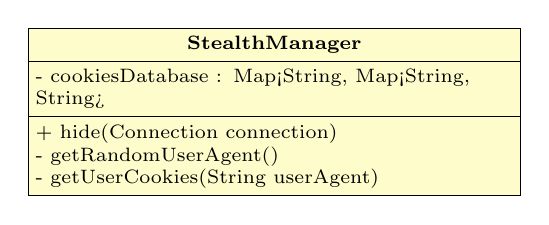
\begin{tikzpicture}
            \begin{class}[text width=0.5\linewidth]{StealthManager}{0,0}
                \scriptsize
                \renewcommand{\umltextcolor}{black}
                \renewcommand{\umldrawcolor}{black}
                \attribute{- cookiesDatabase : Map<String, Map<String, String>}
                \operation{+ hide(Connection connection)}
                \operation{- getRandomUserAgent()}
                \operation{- getUserCookies(String userAgent)}
            \end{class}
        \end{tikzpicture}
\end{figure}
Our \textsc{StealthManager} class is a layer between every connecting class and \url{wg-gesucht.de} (see \textit{Figure} \ref{fig:sec_lay}). It anonymizes every connection by randomly picking an entry from a list with 50 common user agents (\textit{getRandomUserAgent()} method). 
\begin{wrapfigure}{r}{0.54\textwidth}
    \centering
    \includegraphics[width=\linewidth]{images/SecurityLayer.png}
    \caption{\UML Package Diagram showing the security layering}
    \label{fig:sec_lay}
\end{wrapfigure}%
An user agent string is used by web browsers to provide information about the connecting device. This way, websites can provide special representations for e.g. smartphones but it enables also to track suspicious users.\\
The \textsc{StealthManager} class ensures consistency by providing an own cookie database for every user agent, simulating distinct users. Also, it internally adds certain cookies to the databases used by the website to mark users which already passed the security warning and captcha test.
Other classes connect to the website through the \textit{hide(Connection connection)} method, which delays incoming queries for a random amount of seconds. A \textit{Connection} is an object type used by the \textit{JSoup} package consisting an URL.


\subsubsection{CityCrawler}


Our class \textsc{CityCrawler} is used to fetch the HTML pages with offer listings from the website \url{wg-gesucht.de}. It is callable either through the \textit{updateAll()} method to fetch and update all known cities (and thus \textit{maxPages} pages in every city) or through the \textit{updateCityList()} method, which takes an ArrayList with cityIDs as an argument.\\
Every city page has an unique ID (e.g. Munich has the ID 90), which can be extracted by URL manipulation. The \textit{maxCities} integer provides the maximal cityID (used by \textit{updateAll()} method) and the \textit{cities} HashMap provides a mapping of known cityID - city name pairs. This is needed to avoid repeatedly using a wrong URL when connecting to city pages and thus increasing the hazard of being detected as a bot. Connections to the website are processed by the \textsc{StealthManager} class for the same reason.

\begin{figure}[H]
    \centering
    \begin{subfigure}{.35\textwidth}
    \centering
    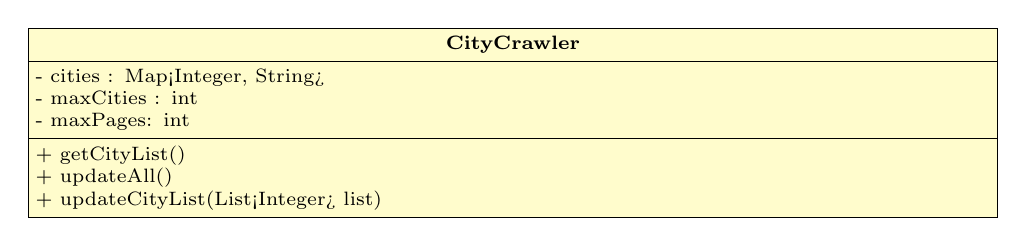
\begin{tikzpicture}
        \begin{class}[text width=1\linewidth]{CityCrawler}{0,0}
            \renewcommand{\umltextcolor}{black}
            \renewcommand{\umldrawcolor}{black}
            \scriptsize
            \attribute{- cities : Map<Integer, String>}
            \attribute{- maxCities : int}
            \attribute{- maxPages: int}
            \operation{+ getCityList()}
            \operation{+ updateAll()}
            \operation{+ updateCityList(List<Integer> list)}
        \end{class}
    \end{tikzpicture}
    \end{subfigure}
    %
    \begin{subfigure}{.59\textwidth}
    \raggedleft
    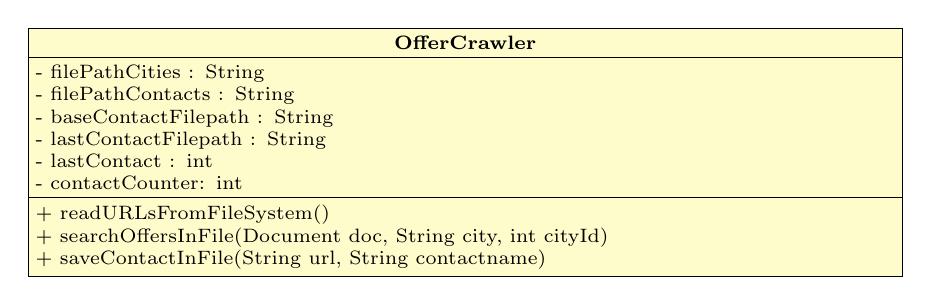
\begin{tikzpicture}
        \begin{class}[text width=.9\linewidth]{OfferCrawler}{0,0}
            \renewcommand{\umltextcolor}{black}
            \renewcommand{\umldrawcolor}{black}
            \scriptsize
            \attribute{- filePathCities : String}
            \attribute{- filePathContacts : String}
            \attribute{- baseContactFilepath : String}
            \attribute{- lastContactFilepath : String}
            \attribute{- lastContact : int}
            \attribute{- contactCounter: int}
            \operation{+ readURLsFromFileSystem()}
            \operation{+ searchOffersInFile(Document doc, String city, int cityId)}
            \operation{+ saveContactInFile(String url, String contactname)}
        \end{class}
    \end{tikzpicture}
    \end{subfigure}
\end{figure}

\subsubsection{OfferCrawler}
\begin{wrapfigure}{r}{0.57\textwidth}
    \centering
    \includegraphics[width=\linewidth]{images/CityOfferCrawler.jpg}
    \caption{Example of a website downloaded by the \textsc{CityCrawler} and an offer extracted by the \textsc{OfferCrawler}.}
    \label{fig:offer_site}
\end{wrapfigure}%
Our class \textsc{OfferCrawler} is used to extract all the offers from the HTML pages that the \textsc{CityCrawler} has downloaded previously. For that it simply iterates through all the saved HTML files in the directory specified by \textit{filePathCities} and searches for a specific headline that every offer in \url{www.wg-gesucht.de} has. However, the headline for advertisements from partner websites differs from mentioned headline, so we did not have to take care of filtering those. The \textsc{OfferCrawler} connects with the URL in every offer and downloads the page to the folder specified in \textit{filePathContacts}. An example for this procedure is given in \textit{Figure} \ref{fig:offer_site}. To cover and resume the offer extraction after an unexpected crash of the program, the \textsc{OfferCrawler} saves the count of the last offer found in a file on the hard drive.

\subsubsection{OfferFilter}
\begin{figure}[H]
        \centering
        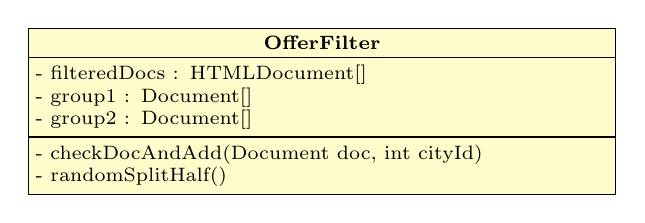
\begin{tikzpicture}
            \begin{class}[text width=0.6\linewidth]{OfferFilter}{0,0}
                \scriptsize
                \renewcommand{\umltextcolor}{black}
                \renewcommand{\umldrawcolor}{black}
                \attribute{- filteredDocs : HTMLDocument[]}
                \attribute{- group1 : Document[]}
                \attribute{- group2 : Document[]}
                \operation{- checkDocAndAdd(Document doc, int cityId)}
                \operation{- randomSplitHalf()}
            \end{class}
        \end{tikzpicture}
\end{figure}
We couldn't use every offer that the \textsc{OfferCrawler} extracted, as some of the offers preemptively excluded persons of certain genders and age groups. Our two personas (as defined in the \textit{.properties} file generated by \textsc{PersonaCreator}) are male and 22 years old, so we had to filter any offer that wouldn't accept them. The \textsc{OfferFilter} takes the output of the \textsc{OfferCrawler} and searches the offer description for the genders and age boundaries the lessors are willing to accept.           % habs kaputt gemacht :-(    \( ͡° ͜ʖ O)/
This information is always found under specific headlines in the offers of \url{www.wg-gesucht.de}, so we hadn't to search the whole text for mentions of age and gender. Also, the \textsc{OfferFilter} discards offers if the contact form is inaccessible. After filtering the offers, the \textsc{OfferFilter} splits those randomly into two preferably equally sized groups.

\subsubsection{MessageWriter}
\label{sec:messagewriter}
\begin{figure}[H]
        \centering
        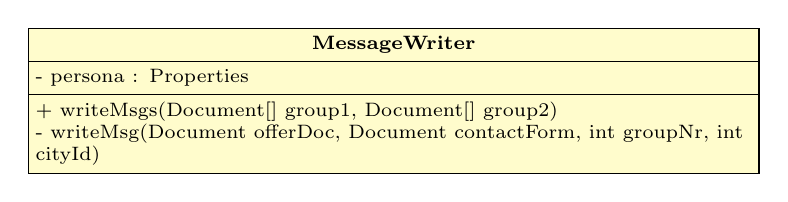
\begin{tikzpicture}
            \begin{class}[text width=0.75\linewidth]{MessageWriter}{0,0}
                \scriptsize
                \renewcommand{\umltextcolor}{black}
                \renewcommand{\umldrawcolor}{black}
                \attribute{- persona : Properties}
                \operation{+ writeMsgs(Document[] group1, Document[] group2)}
                \operation{- writeMsg(Document offerDoc, Document contactForm, int groupNr, int cityId)}
            \end{class}
        \end{tikzpicture}
\end{figure}
The \textsc{MessageWriter} takes the two sets (realised as an enumeration class) that the \textsc{OfferFilter} has created and writes the respective applications. This is done by using the application text (see \ref{sec:setup}) which previously has been saved on the hard drive by the \textsc{PersonaCreator}. The name of the lessor can be extracted from the contact form on the offer page. The resulting text is saved on the hard drive and could be checked manually before executing the \textsc{MessageSender}. \newline
We decided to send two different kinds of messages - formal ones and and informal ones - as we assumed that different persons would expect different salutations. Our idea was to decide what kind of message to write based on whether they gave their last name or not. Persons that only gave their first name received an informal message. In most cases, the gender of the person can be found out by examining the label of the profile picture of the lessor (there is either a male or female profile picture). In all other cases we chose a gender neutral salutation. This resulted in the following possible salutations:

\begin{itemize}
    \item Hallo \_\_, (gender neutral)
    \item Sehr geehrte Frau \_\_, (female, formal)
    \item Sehr geehrter Herr \_\_, (male, formal)
    \item Liebe \_\_, (female, informal)
    \item Lieber \_\_, (male, informal)
\end{itemize}

Unfortunately, the division into formal and informal message groups did not seem to be very successful, as some of the lessors reacted with confusion to the formal salutations.
\newpage
\subsubsection{MessageSender}
\begin{figure}[H]
        \centering
        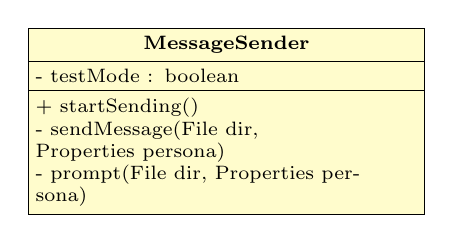
\begin{tikzpicture}
            \begin{class}[text width=0.4\linewidth]{MessageSender}{0,0}
                \scriptsize
                \renewcommand{\umltextcolor}{black}
                \renewcommand{\umldrawcolor}{black}
                \attribute{- testMode : boolean}
                \operation{+ startSending()}
                \operation{- sendMessage(File dir, Properties persona)}
                \operation{- prompt(File dir, Properties persona)}
            \end{class}
        \end{tikzpicture}
\end{figure}
The \textsc{MessageSender} is responsible for the final step of the process: it accesses the contact form by searching for certain tags in every offer selected by the \textsc{OfferFilter} and fills the 'send a message'-form with data generated by the \textsc{PersonaCreator} and \textsc{MessageWriter}. Also it makes sure to request a copy of the application via e-mail, so that we could double-check that the right amount of applications was sent.\\
In addition, it consists of a special mode for testing purposes and a prompt option, which asks to try again in case of a failure (e.g. broken internet connection).

\section{The Experiment}
\subsection{Setup}
\label{sec:ex_setup}
Our initial hypothesis stated that there is a positive correlation between the amount of right wing party voters in a certain city and it's \textit{racism score}, calculated by comparing the success of the two almost identical profiles on \url{www.wg-gesucht.de}. Our goal was to show that a foreign name makes you less successful in finding accommodation. To exclude any other possible reason for rejection, we decided to vary only the foreign tone of the name in both personas. Finally, we came up with \textit{Sebastian Winkler} and \textit{Achmet Bukhari} and the following flat share offer request:\\

\footnotesize\raggedleft
\begin{tabular}{|p{.9\textwidth}}
Hallo \_\_,\\ mein Name ist \_\_ und ich studiere im 3. Semester Maschinenbau. Zurzeit bin ich 22 Jahre alt (werde aber bald 23) und suche im Moment nach einer netten Wohngemeinschaft. Ich bin Nichtraucher und habe keinerlei (mir bekannten) Allergien. In meiner Freizeit mache ich gerne Sport (im Winter Skilaufen, sonst Volleyball, 'Fitnessstudio') und spiele Gitarre (keine Sorge, nicht daheim, nur mit meiner Band im Bandproberaum). Außerdem koche ich ab und zu gerne (meine Freunde empfehlen mich weiter (: ). Ich würde mir gerne die Wohnung mal anschauen, aber ich kann dir auch erst mehr Informationen zu mir senden wenn gewollt. (Facebook, Telefonnummer). \\ Ich würde mich freuen von dir zur hören! \\ Beste Grüße, \_\_.\\
\end{tabular}\\
\normalsize
\bigskip
\raggedright
The text differs depending on whether the message was classified as formal or informal (see \ref{sec:messagewriter}).
\newpage
Furthermore, we chose seven German cities to conduct our experiment by searching the results of the last Bundestag elections \cite{Bun:1} for cities meeting two criteria:

\begin{enumerate}
    \item Relatively extreme percentage (low or high) of \textit{AfD}\footnote{\textit{Alternative für Deutschland} is a populist party, which achieved 12,6\% of all votes at the Bundestag election in 2017} voters
    \item High usage of \url{www.wg-gesucht.de} for housing market purposes (at least 40 flat share offers within a week)
\end{enumerate}

We selected the following cities:

\begin{figure}[H]
    \centering
    \begin{subfigure}{.4\textwidth}
    \centering
 \begin{tabular}{!{\vrule width 3pt}l c!{\vrule width 3pt}}
 \hline
 \rowcolor{black!0}
 Name & AfD percentage \\ [0.7ex] 
 \hline\hline
 \rowcolor{green!30}
 Münster & 4.9\% \\ 
 \hline
 \rowcolor{green!25}
 Osnabrück & 7.3\% \\
 \hline
 \rowcolor{green!20}
 München & 8.4\% \\
 \hline\hline
 \rowcolor{blue!15}
 Erfurt & 18.2\% \\
 \hline
 \rowcolor{blue!20}
 Leipzig & 18.3\% \\ 
 \hline
 \rowcolor{blue!25}
 Dresden & 23.2\% \\
 \hline
 \rowcolor{blue!30}
 Chemnitz & 24.3\% \\ [0.5ex] 
 \hline
\end{tabular}
\end{subfigure}
\begin{subfigure}{0.59\textwidth}
\centering
\includegraphics[width=\linewidth]{images/Deutschland.png}
\end{subfigure}
\end{figure}

Therefore, we had two independent variables, namely, whether we used the foreign or the German profile name, and the percentage of \textit{AfD} voters. The dependent variable was the degree of positive responses we got. We used an own email address at \textit{gmx.de} for every city/persona combination in accordance to the following pattern: \textit{forename.surname.cityID@gmx.de}\\
\newpage
To increase reliability, we classified the emails into distinct folders with the following codebook:
\begin{center}
\resizebox{\textwidth}{!}{%
 \begin{tabu}{!{\vrule width 3pt} p{0.25\linewidth} !{\vrule width 3pt} p{0.25\linewidth} !{\vrule width 3pt} p{0.25\linewidth} !{\vrule width 3pt} p{0.25\linewidth} !{\vrule width 3pt}}
 \hline
 \rowfont{\centering}\cellcolor{green!20}Positive answer & \cellcolor{red!20}Negative answer & \cellcolor{yellow!20}Personal check & \cellcolor{blue!20}Excluded answer\\ [0.5ex] 
\hline\hline
\rowfont{\small}
 Mentioning time and place of house viewing \vspace{3pt}& Apologising for already giving the room away &  Asking for a link to Facebook profile & Checking correct understanding of offer \\
 \hline
 \rowfont{\small}
 Asking for a time frame for the house viewing \vspace{3pt} & No answer at all & Asking for current employment  & Asking for subletting secretly\\
 \hline
 \rowfont{\small}
 Providing or asking for a phone number for meeting purposes \vspace{3pt}& & Asking for a residence permit / photos /  	certificate of bond &\\
\hline
\end{tabu}}
\end{center}

Our automatic tool crawls recent offers from a chosen city and randomly splits them into two groups. Thus, every offer has the same chance to be selected into either group. This two offer bundles get transformed to message bundles, which then are sent using the form on each offer site.\\
Exactly one week after the process of sending the messages, we logged into the related mailboxes and classified every email using our codebook. E-mails arriving after classification got discarded and did not influence our statistics.

Until 8th of January 2018 we made preparations and wrote the tool. Within a time frame of 5 days we started sending the messages. On 20th January we classified the last email and started analysing the results.

\subsection{Results}
\begin{figure}[H]
\centering
\resizebox{.6\textwidth}{!}{%
\begin{tikzpicture}
\begin{axis}[
    ylabel={positive response per message sent},
    ylabel style = {font = \LARGE},
    enlargelimits=0.15,
    legend style={at={(0.5, -0.15)},
    anchor=north, legend columns=-1},
    symbolic x coords={Münster,Osnabrück,München,Erfurt,Leipzig,Dresden,Chemnitz},
    ybar,
    xtick=data,
    width=\textwidth,
    x tick label style = {font = \Large, rotate = 25},
    bar width=18pt,
    visualization depends on=y \as \rawy,
    nodes near coords align={vertical},
    every node near coord/.append style={font=\footnotesize, /pgf/number format/fixed, shift={(axis direction cs:0,-\rawy)}, yshift=-12pt},
    %set layers,% using layers
    %mark layer=axis tick labels% defines the layer of the marks
    ]
    \addplot+[nodes near coords] coordinates {
    (Münster, 0.2745) (Osnabrück, 0.5536) (München, 0.1607) (Erfurt, 0.3333) (Leipzig, 0.4839) (Dresden, 0.359) (Chemnitz, 0.75)};
    
    \addplot+[nodes near coords] coordinates {
    (Münster, 0.2308) (Osnabrück, 0.4386) (München, 0.0686) (Erfurt, 0.3158) (Leipzig, 0.25) (Dresden, 0.28) (Chemnitz, 0.3333)};
    
    \addplot[blue,sharp plot,style = thick,dash dot] coordinates {(Münster, 0.2877) (Osnabrück, 0.2877) (München, 0.2877)}
;
    \addplot[red,sharp plot,style = thick,dash dot] coordinates {(Münster, 0.2085) (Osnabrück, 0.2085) (München, 0.2085)}
;
    \addplot[blue,sharp plot,style = thick,dash dot]
coordinates {(Erfurt, 0.432) (Leipzig, 0.432) (Dresden, 0.432) (Chemnitz, 0.432)}
;
    \addplot[red,sharp plot,style = thick,dash dot]
coordinates {(Erfurt, 0.29) (Leipzig, 0.29) (Dresden, 0.29) (Chemnitz, 0.29)}
;

    \coordinate (A) at (axis cs:Münster,0.2447);
    \coordinate (B) at (axis cs:Münster,0.355);
    \coordinate (O1) at (rel axis cs:0,0);
    \coordinate (O2) at (rel axis cs:1,0);
    
    \draw[red,sharp plot,style=ultra thick,dash pattern={on 4pt off 10pt}] (A -| O1) -- (A -| O2);
    \draw[blue,sharp plot,style=ultra thick,dash pattern={on 4pt off 10pt}] (B -| O1) -- (B -| O2)node [pos=0.44,yshift=8pt,black]{Overall response};

    \legend{Sebastian\quad\ , Achmet}
\end{axis}
\end{tikzpicture}}
\caption{Results in all cities in ascending \textit{AfD} percentage order.}
\label{results}
\end{figure}

By looking at the responses we could see that our persona with the foreign name (\textit{Achmet Bukhari}, 24.5\% positive responses) received 10.5\% less positive answers than the one with the German name (\textit{Sebastian Winkler}, 35.0\% overall positive responses). Furthermore it is evident, that it becomes less likely to receive an answer (be it positive or negative) to a request with an increasing number of inhabitants in the city where the request is sent. The gap between positive answers for \textit{Sebastian Winkler} is higher in cities with a high percentage of \textit{AfD}-supporters (> 18.5\%) than in cities with a low percentage (< 8.5\%).
\subsection{Problems}
As already mentioned in section \ref{sec:setup}, one big obstacle we had to overcome was the website's bot checker. Our \textsc{StealthManager} component made sure that the program paused for a random amount of time -- between 8 and 18 seconds -- before connecting to the website and randomly chose different user agents. Still the bot checker blocked us after about one hundred connections to the website which required us to manually change the VPN server which we used for connecting. \newline
The long waiting time between every connection raised another issue: our program had to run for several hours to send a few hundred applications. To avoid losing all progress in case of a crash of the program we decided to save the results of every component on the hard drive. This also allowed us to interrupt the program and to check the results manually before proceeding.

\subsection{Ethical Considerations}
Reflecting the answers we got, we filled seats on house viewing events which could have been given to real people. Also, we got answers from stakeholders, who invited us exclusively on a specific date. We could have saved them a lot of time, if we had arranged an automatic reply on all mail boxes beforehand, informing the stakeholders about the study or politely declining the invitation.\\
In addition, it should be noted, that our experiment may have violated the terms and conditions of \url{wg-gesucht.de}. Before and during the experiment, we took actions to conceal our identity, but in our estimation, our program barely had an effect on the performance of the website or it's user experience. This aspect should be considered in greater detail when executing bigger studies.

\bibliographystyle{siam}
\bibliography{main}

\end{document}
